%!TEX root = ../main.tex

\section{Cost of Movement}
The movement of a dragline as it moves overburden from the mine to the spoil, this cost of movement has been explored in several papers and as such models used may be adapted. The work presented by B .Erdem and H. Duzgun
suggests that the time taken for a movement is linear to the angle the boom will move \cite{Dmove}. This model was validated against data in the paper and as such could be seen as a reliable model. The data presented in the paper can be seen below in figure \ref{Swingangle},throughout the paper this data is applied for all actions that a dragline can perform across a variety of potential block removal methods, suggesting that an appropriate model for the cost of an action is \(T = k\times \theta + c\) \cite{Dmove} where $k$ and $c$ are constants dependant on the dragline selected. This is further reinforced when all modes of excavation are compared against one another, while an $R^2$ value of 0.7959 \cite{Dmove} is not ideal it will be a reasonably effective model when only one excavation model is considered. It should be noted that this model is also applied in the work of Haoquan Liu who has also used this model in his optimisation of a dragline in a block \cite{A*Search}. 

\begin{figure}[h]
\caption{Swing times as a function of swing angle}
\label{Swingangle}
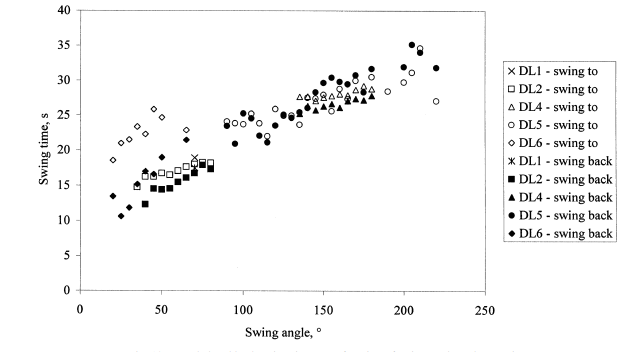
\includegraphics[width=\textwidth]{Swingangle.png}
\end{figure}

\begin{figure}[h]
\caption{Swing times as a function for all modes of excavation.}
\label{Swingangle}
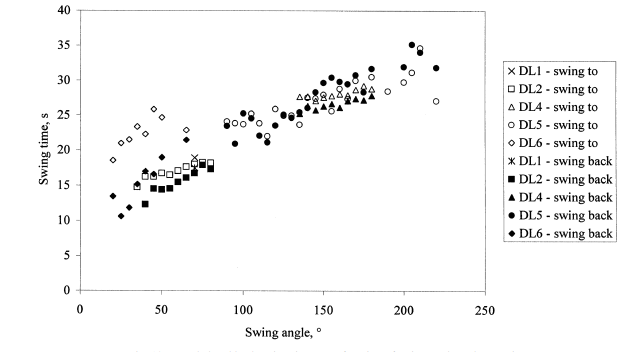
\includegraphics[width=\textwidth]{Swingangle.png}
\end{figure}


\section{Cost of a Block}
The cost of a block is a topic that has been studied and approached in a range of ways, however the thing that all methods have in common is that the method used is a technique found in operations research\cite{A*Search}\cite{PacificCoal}, therefore the models that have been suggested will be split into the appropriate modelling techniques used. Here the consideration is the most efficient way to remove overburden from the block and into the spoil channel. 

\subsection{Linear Programming}
Linear programming is the approach used in the work of  Haoquan Liu for his work on the optimisation of dragline movement through a block, here it is suggested that the model can be solved using mixed integer linear programming\cite{A*Search}. This work shows a method that can determine an optimal solution quickly and with minimal calculations. The formulation of this model is made of a series of constraints and an objective, they are as follows.  \\
At each position the dragline can only move material within its operating radius, there is a minimum and maximum radius that must be observed for the consideration of this reach \cite{ORLeslie}. Other constraints used to describe the motion of the bucket through the mine such that the bucket of the dragline will not travel over crests of overburden\cite{ORLeslie} and that all elements can only be removed if the material preceding them is also removed \cite{ORLeslie}, these constraints are sufficient for the definition of the model of the dragline. 

\subsection{Dynamic Programming}
The method of dynamic programming for the optimisation of dragline movement throughout a block was investigated by Pacific Coal, suggesting the viability of a model of a dragline using dynamic programming.\cite{PacificCoal} For this project it was seen as reasonable to remodel the formulation first considered in this paper however as the formulation required the solving of a partial differential equation at each step of the formulation\cite{PacificCoal}, this was seen as impractical and in fact never ran. This is combined with the fact that the model was only ever considered on paper with no thoughts regarding the applications and algorithmic complexity of such a formulation. This model however did suggest the potential for linearisation and simplifications that if made would result in a solvable and simple dynamic program that could be used for the calculation of dragline block length. 

